\section{Benchmark results}

\subsection{ClustAssess vs Clusim - ECS benchmarks}

\begin{frame}
    \begin{itemize}[<+->]
        \item To provide an appropriate benchmark of the \texttt{ClustAssess} package, we will compare its performance to \texttt{Clusim}. 
        \item \texttt{Clusim} is a Python package that contains the official implementation from the authors of the ECS paper \cite{Gates2019b}.
        \item In \texttt{Clusim}, the ECS between two disjoint partitions is determined by calculating the affinity matrices.
        \item The benchmark is done by performing the ECS between two fixed partitions using the implementations from \texttt{ClustAssess} and \texttt{Clusim}. The size of the partitions varies from 50 to 90 000. The execution is repeated 30 times.
    \end{itemize}
\end{frame}

\begin{frame}{Runtime comparison}
    \begin{columns}
        \begin{column}{0.45\textwidth}
            \justifying
           

           \texttt{ClustAssess} requires less than a second to calculate the ECS, while the execution time of \texttt{Clusim} increases exponentially.
        \end{column}

        \begin{column}{0.5\textwidth}
            \begin{figure}
                % \centering
                % \makebox[\textwidth][c]{
                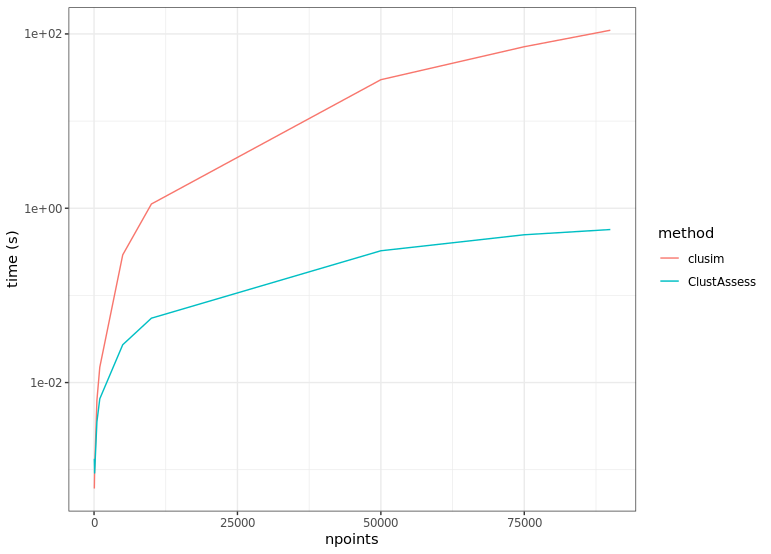
\includegraphics[width=0.95\textwidth]{images/ch4/4_clusim_ca_time.png}
                % }
                
                \caption{\justifying \textbf{Execution time benchmark} The size of the partitions used for the benchmark are displayed on the X-axis. The time (in seconds) required to calculate the ECS using ClustAssess (blue) and Clusim (red) is displayed on the Y-axis. The results are displayed on a logarithmic scale.}

            \end{figure}
        \end{column}
    \end{columns}
\end{frame}

\begin{frame}{Comparison of memory usage}
    \begin{columns}
        \begin{column}{0.45\textwidth}
            \justifying
            % The experiment was repeated to evaluate the memory required by each package to perform the calculation.

            For the optimized version from \texttt{ClustAssess} the data storage scales proportionally to the number of clusters. 
            \bigskip
            
           Memory allocation of $\leq$ 100 MiBs. 
           \bigskip

           The storage of the whole affinity matrix in \texttt{Clusim} is inefficient, reaching a memory allocation of 241 GiBs for the largest dataset.
        \end{column}

        \begin{column}{0.5\textwidth}
            \begin{figure}
                % \centering
                % \makebox[\textwidth][c]{
                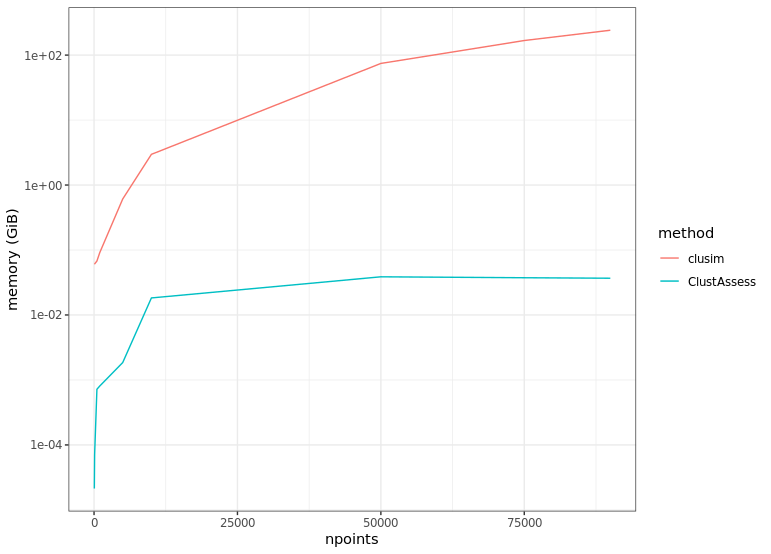
\includegraphics[width=0.95\textwidth]{images/ch4/4_clusim_ca_memory.png}
                % }
                \caption{\justifying \textbf{Memory usage benchmark} The size of the partitions used for the benchmark are displayed on the X-axis. The amount of memory (in GiBs) required to calculate the ECS using ClustAssess (blue) and Clusim (red) is displayed on the Y-axis. The results are displayed on a logarithmic scale.}
            \end{figure}
        \end{column}
    \end{columns}
\end{frame}

\begin{frame}{Performance with varying number of clusters}
    \begin{itemize}
    \item \texttt{ClustAssess} calculates a number of unique ECS values proportional to the number of clusters of both partitions.
        

    \item It is expected that, as the number of clusters increases, the \texttt{ClustAssess} package will require more time and space to calculate the ECS.

    \item \texttt{Clusim} calculates the whole affinity matrix, so its performance shouldn't be affected by the number of clusters.

    \end{itemize}
\end{frame}

\begin{frame}{Performance with varying number of clusters}
    \begin{figure}
        \centering
        \begin{subfigure}[t]{0.47\textwidth}
            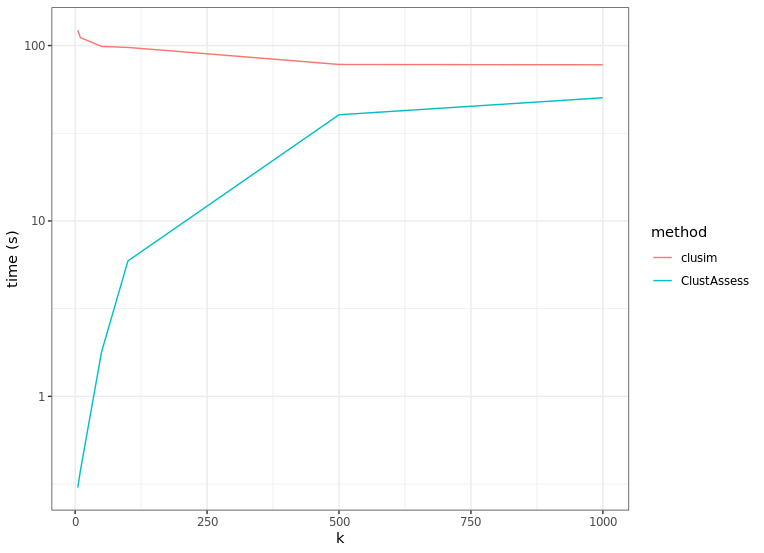
\includegraphics[width=\textwidth]{images/ch4/4_clusim_ca_time_k.png}
        \end{subfigure}
        \begin{subfigure}[b]{0.47\textwidth}
            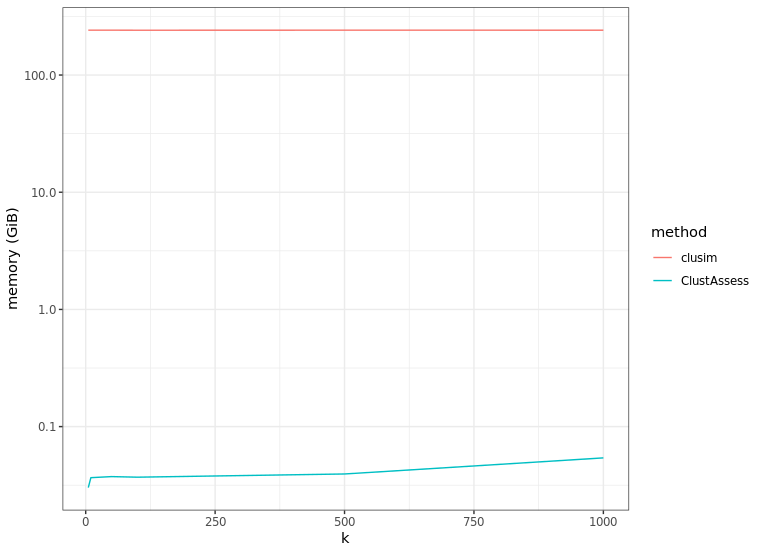
\includegraphics[width=\textwidth]{images/ch4/4_clusim_ca_memory_k.png}
        \end{subfigure}
        \caption{\textbf{Performance comparison for different number of clusters} Left panel - the median time of execution (in seconds) measured after 30 runs for ClustAssess (blue) and Clusim (red). Right panel - the median memory usage (in GiB) measured after 30 runs for ClustAssess (blue) and Clusim (red). The results are displayed on a linear scale.}
    \end{figure}
\end{frame}

\subsection{Stability pipeline benchmarks}

\begin{frame}{How the stability pipeline will be benchmarked}
    \begin{itemize}[<+->]
        \item We will evaluate the performance of the five independent components that provide the data for the plots: \texttt{feature\_stability}, \texttt{nn\_n\_conn\_comps}, \texttt{nn\_importance}, \texttt{clustering\_importance}, \texttt{resolution\_importance}.
        \item The stability pipeline will be evaluated on the Mende data \cite{Mende2022} with subsamples ranging from 1000 to 13000 cells.
        \item The pipeline allows support for parallelisation, so we will measure the pipeline's performance by varying the number of cores.
        \item We will also evaluate the impact of using different ECS threshold values: 1, 0.99 and 0.95.
    \end{itemize}
\end{frame}

\begin{frame}
    \begin{figure}
                % \centering
                % \makebox[\textwidth][c]{
                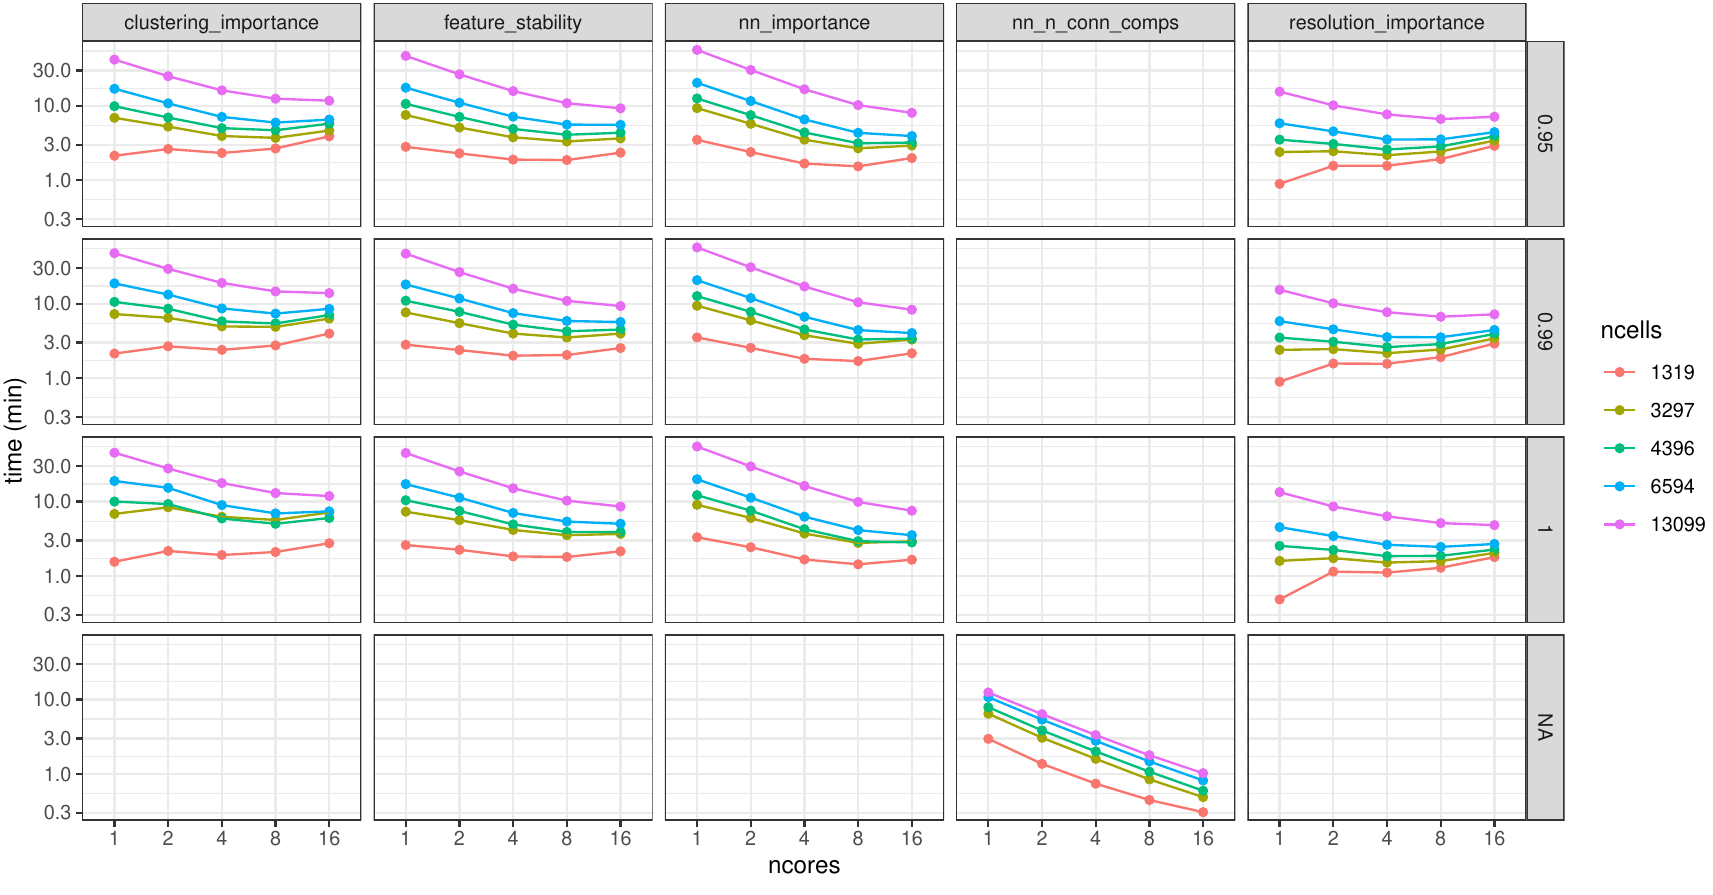
\includegraphics[width=0.8\textwidth]{images/ch4/4_pipeline.png}
                % }
                \caption{\justifying \textbf{Stability pipeline runtime benchmark} The column designate a different component involved in the pipeline. The rows indicate different ECS threshold values. On the X-axis we represent different number of cores. The Y-axis contains the time required (in minutes) for the execution. The colour indicates the size of the dataset.} %We observe no performance gain when ECS threshold is lowered. \texttt{nn\_n\_conn\_comps} has the best scaling when increasing the dataset, followed by \texttt{resolution\_importance}. Adding more cores generally brings a performance boost, with some exceptions related to the overhead created by either the small size of the dataset or the ratio between the number of runs and the number of cores. }
            \end{figure}
\end{frame}